\subsection{Struktura Nadređeni-Podređeni}

Struktura Nadređeni-Podređeni (eng. Master-Slave) je koncept, odnosno model, u kojem je ostvarena unarna komunikacija \footnote{Komunikacija u jednom smjeru}. Koncipirana je na takav način da je jedan uređaj Nadređeni, a drugi (ili više drugih uređaja) su Podređeni. Tako da jedan uređaj "naređuje", a ostali uređaji bez pogovora, obavljaju posao. U ovom radu se ova struktura iskoristila na način da je \textit{Raspberry Pi} bio povezan sa \textit{Arduino Uno} kontrolerom. Povezivanje se ostvarilo preko USB portova, tako da se komunikacija odvija serijskim putem.\\
U ovom slučaju \textit{Raspberry Pi} je Nadređeni, a \textit{Arduino Uno} Podređeni. Na taj način se \textit{Raspberry Pi} oslobodio "razmišljanja" o tome kako pojedine komponente rade, time je omogućena bolja obrada prikupljenih podataka. Na temelju obrade podataka \textit{Raspberry Pi} šalje odgovarajuće poruke \footnote{VIDI STRANICU KOMUNIKACIJA}, putem serijskog porta, \textit{Arduino Uno} kontroleru; koji se ponaša u skladu sa poslanom porukom.\\
Na sljedećoj slici je prikazan spoj dvaju uređaja preko USB kabela.
\begin{figure}[h]
    \centering
    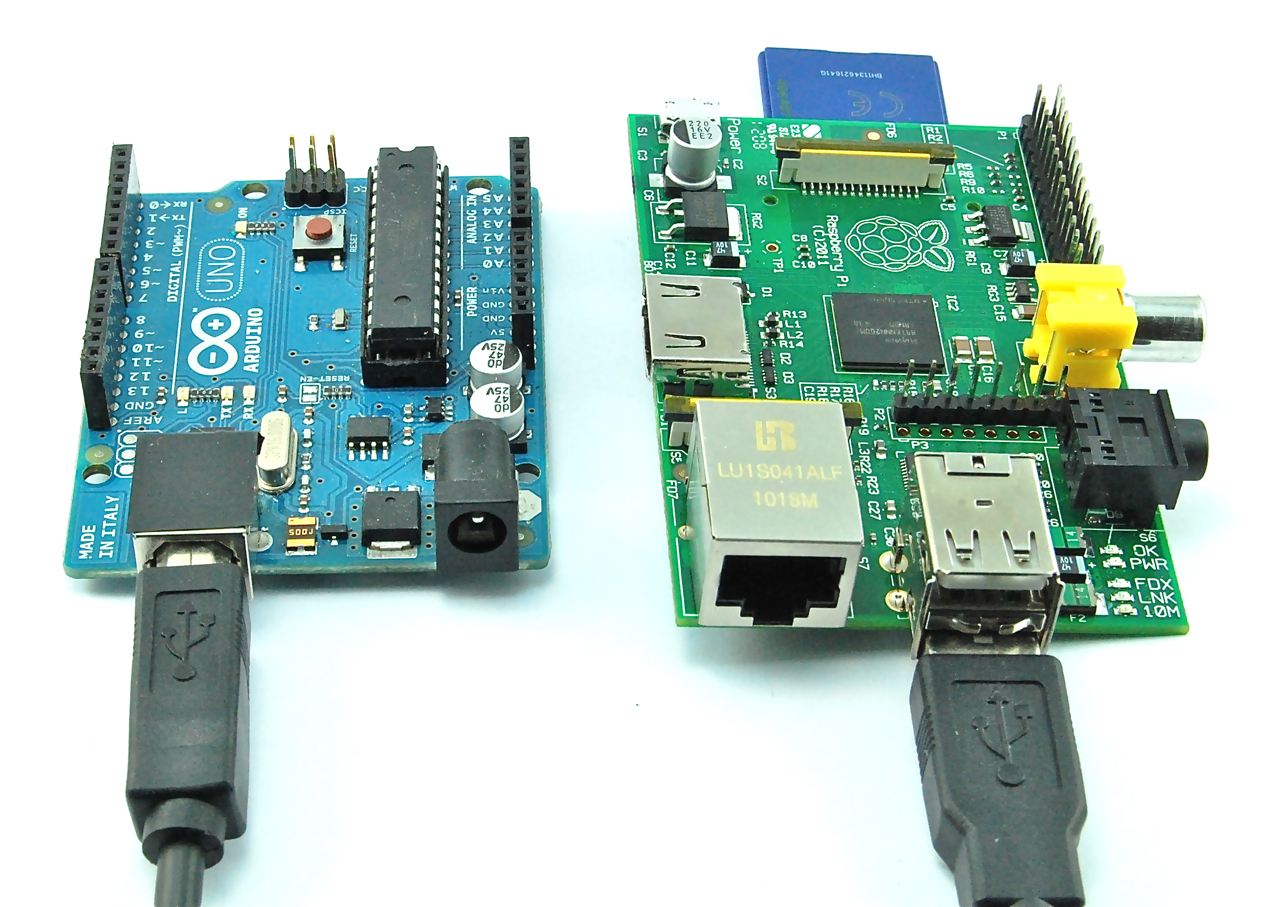
\includegraphics[width=0.5\textwidth]{master_slave.jpg}
    \caption{USB konekcija \textit{Raspberry Pi} sa \textit{Arduino Uno}}
    \label{fig:mesh1}
\end{figure}
\\
